\documentclass{scrartcl}

\usepackage[T1]{fontenc}
\usepackage[utf8]{inputenc}

\title{Mobile Dev Week 3 Lab}
\author{Daniel Coady (102084174)}
\date{02/09/2019}

\usepackage{graphicx}

\begin{document}

\maketitle

\section*{Food Parcels}
\subsection*{Task 1}
\begin{figure}[h]
    \centering
    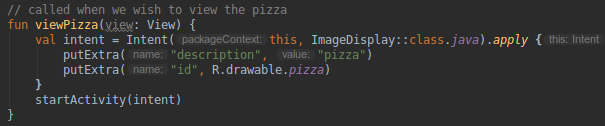
\includegraphics[scale=0.6]{images/screen1.png}
    \caption{The code that allows the  two activities to connect with each other}
\end{figure}

To allow for each activity to communicate with each other for consistency across the app,
we can use intents. With intents we are able to declare what activity we wish to be able to
move onto as well as the data that should go along with it. In this case we are able to send
a description and the id of the photo that has been touched so that we can show a larger version
of it along with it's short description.

\pagebreak

\begin{figure}[h]
    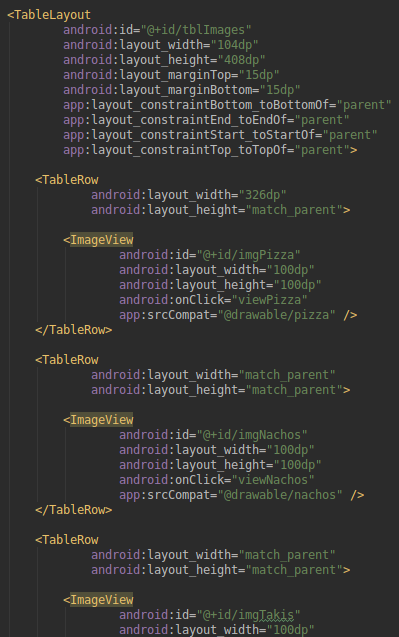
\includegraphics[scale=0.5]{images/screen2.png}
    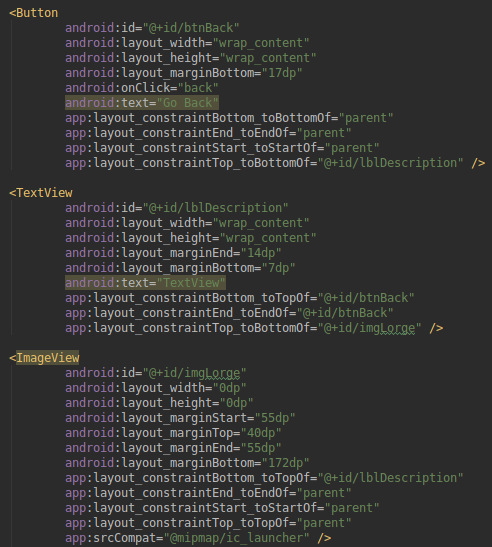
\includegraphics[scale=0.5]{images/screen3.png}
    \caption{Part of the XML used for the activities}
\end{figure}

\pagebreak

\begin{figure}[h]
    \centering
    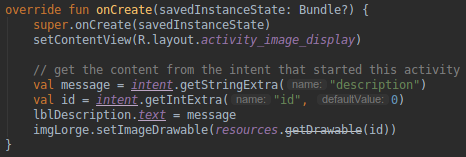
\includegraphics[scale=0.6]{images/screen4.png}
    \caption{Code used to set the views in the image view activity}
\end{figure}

Here we are now collecting the information stored in the intent from the previous activity to
display the information requested.

\pagebreak

\begin{figure}[h]
    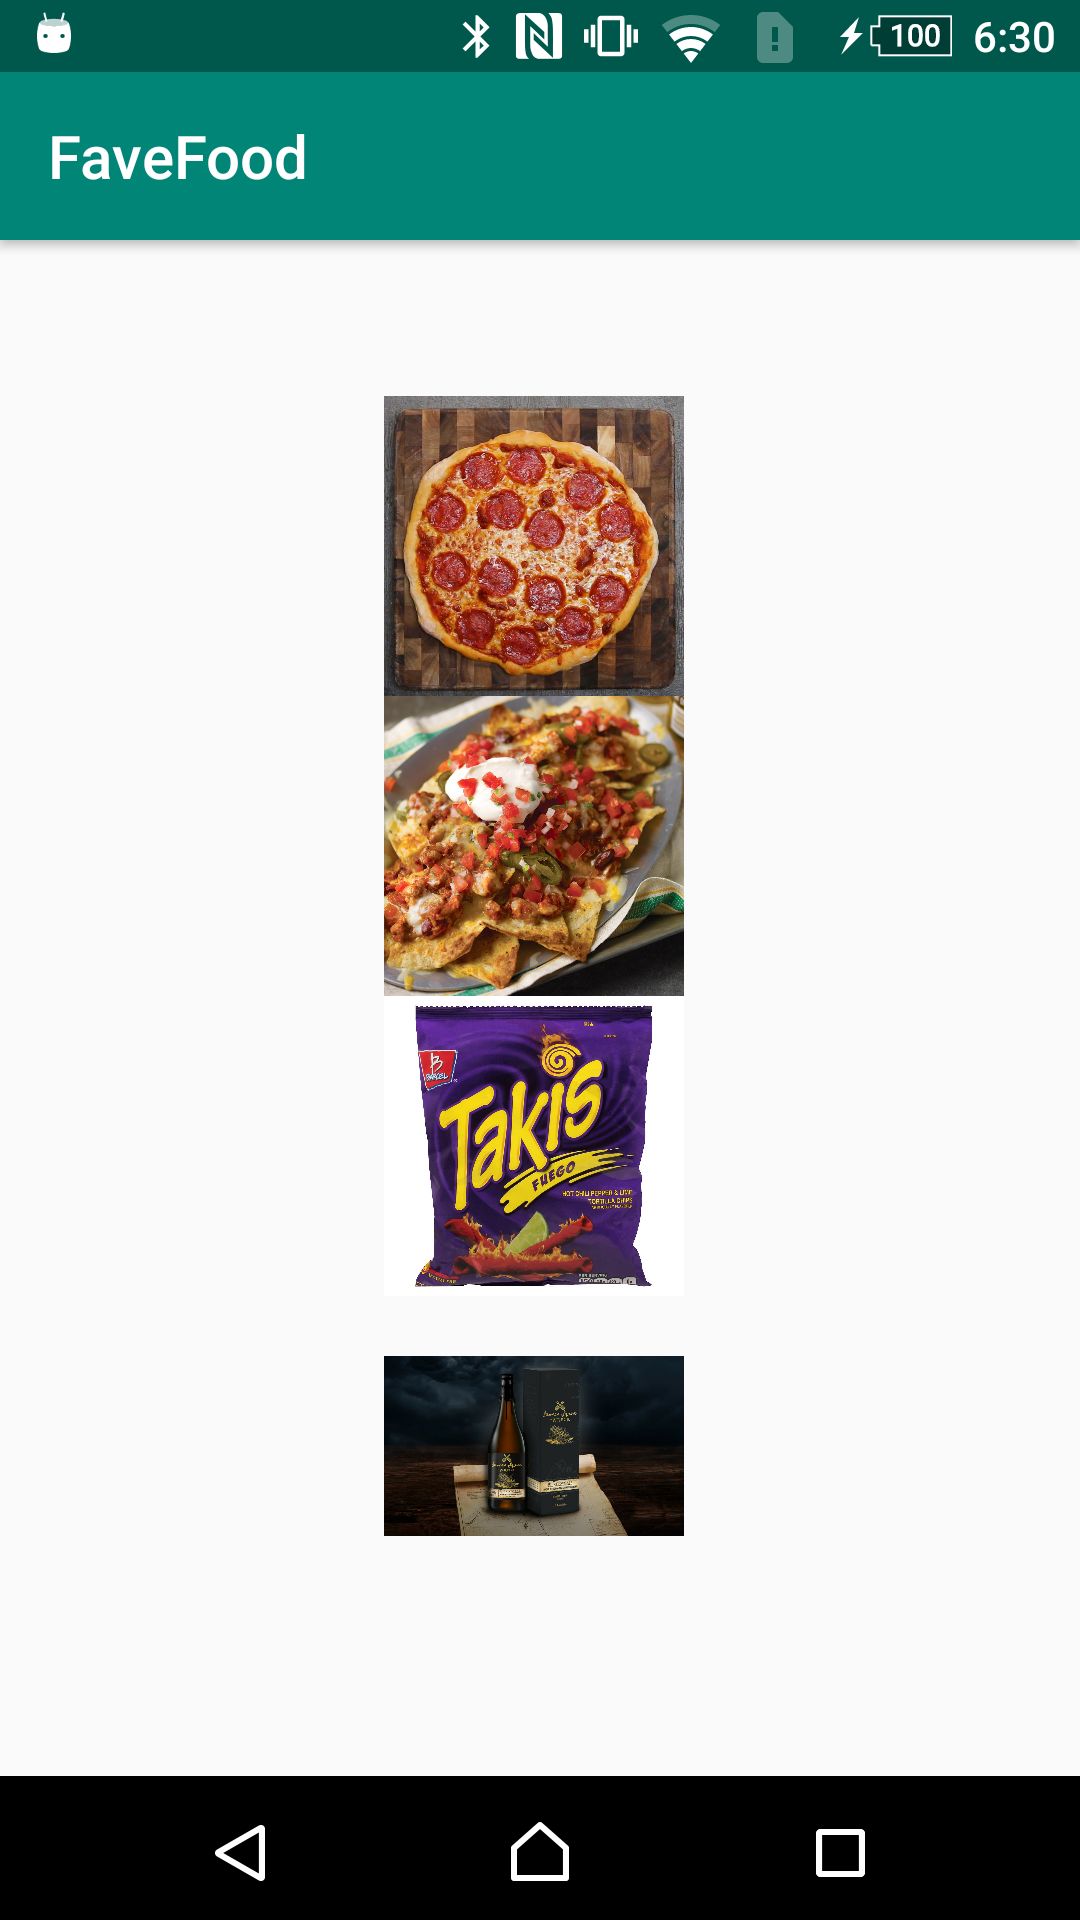
\includegraphics[scale=0.2]{images/screen5.png}
    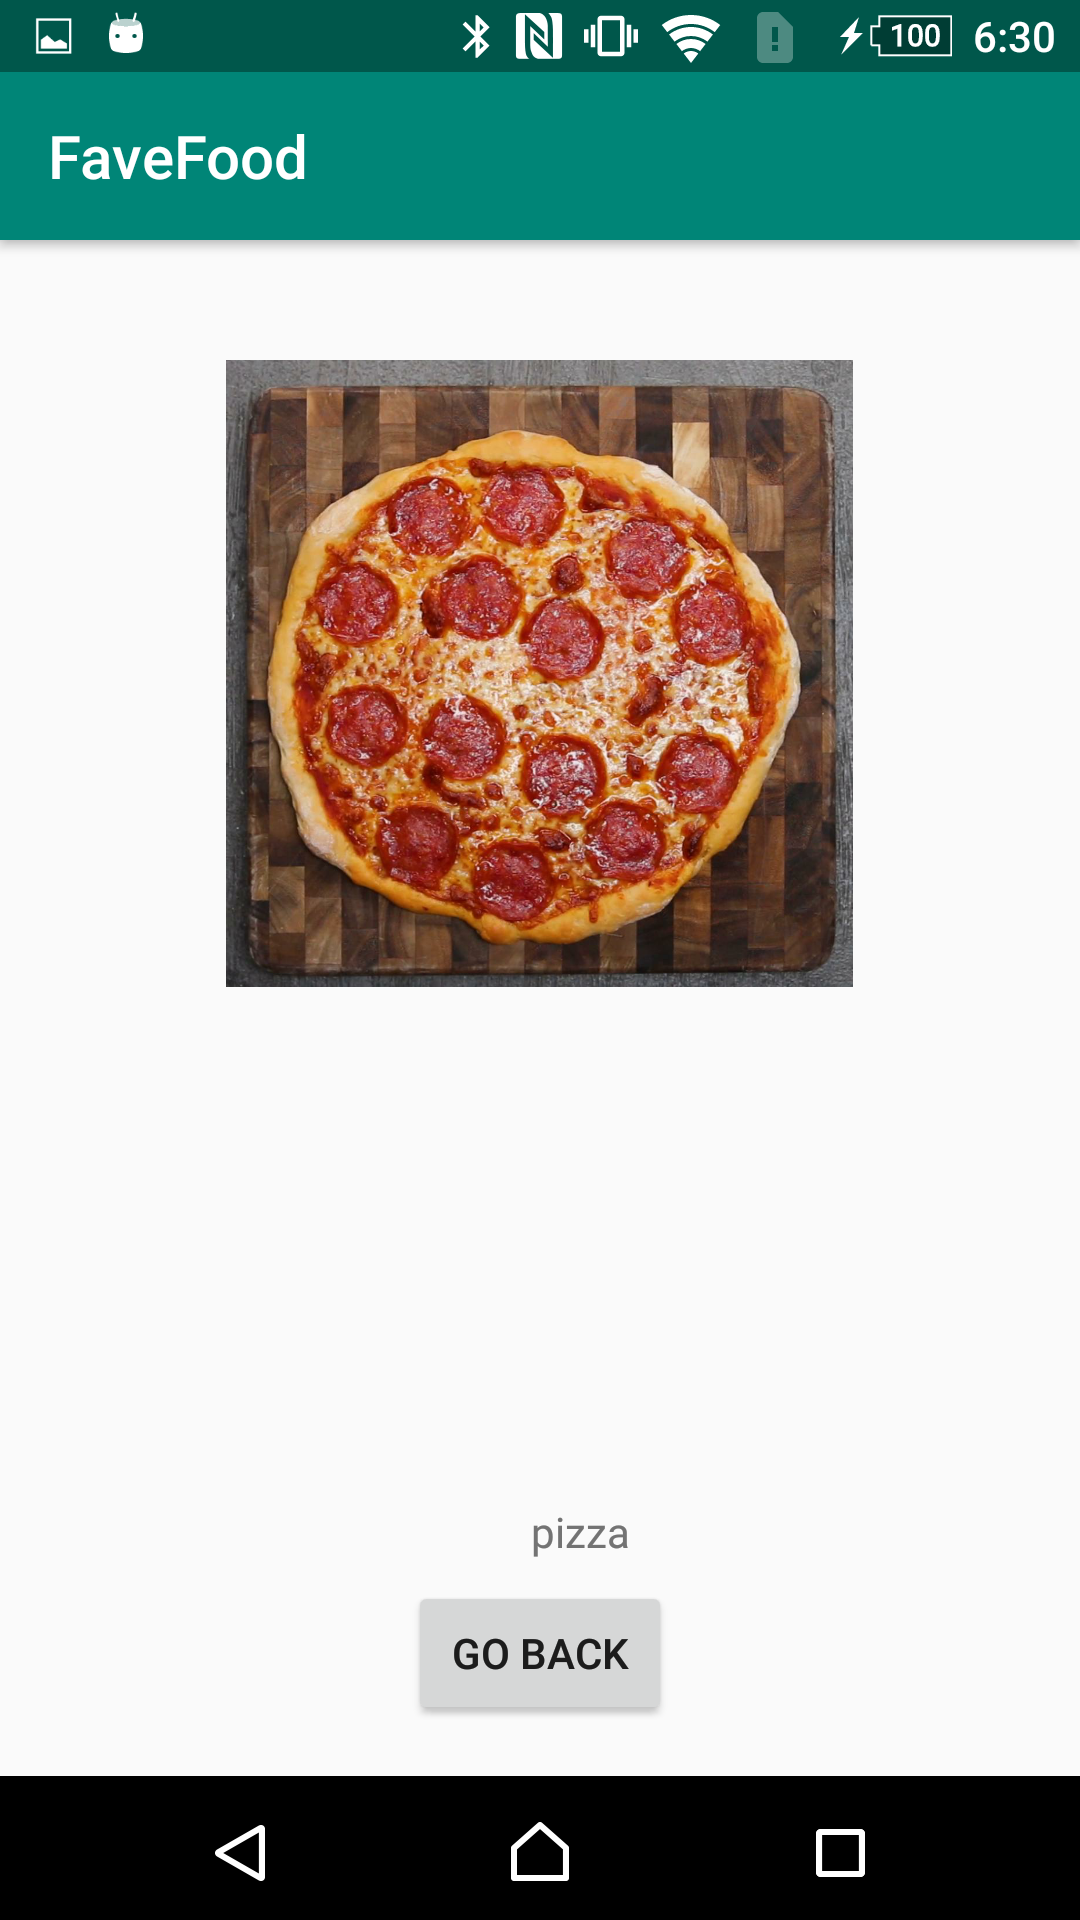
\includegraphics[scale=0.2]{images/screen6.png}
    \caption{The application in action}
\end{figure}

\pagebreak

\subsection*{Task 2}

\end{document}
